\chapter{{\iqist}简介}
\label{chap:intro}

本章将让用户对{\iqist}软件包有一个初步的了解,适合此前从未接触过{\iqist}的
用户阅读。在第\ref{chap:install}章至第\ref{chap:sci}章,将着重描述{\iqist}
的量子杂质求解器组件的具体用法,资深用户可以选择性阅读。在第\ref{chap:tools}
章,将介绍{\iqist}的辅助工具组件的用法,资深用户可以选择性阅读。
第\ref{chap:application}章中包含了若干个深入浅出的计算实例以及项目实战解析,
可供用户学习参考。在本文文末还提供了一个简短的附录,收集了用户经常会遇到的
问题并给出解答。

\section{什么是{\iqist}?}
\label{sec:whatisit}

{\iqist}是{\color{red}I}nteracting {\color{cyan}Q}uantum {\color{cyan}I}mpurity {\color{cyan}S}ystems 
Simulating {\color{cyan}T}oolkit(相互作用量子杂质系统模拟工具包)的英文字头
缩写。顾名思义,{\iqist}是由我们独立开发的,若干个用于处理不含时相互作用量
子杂质模型的软件的集合。这些软件包括了十余种量子杂质模型求解器以及配套的前
处理软件和后处理程序,是动力学平均场理论框架中最为核心的部分。

{\iqist}软件包的主要部分是黄理博士\footnote{亦即本用户手册的第一作者。}在中
国科学院物理研究所理论室T03组攻读理论物理专业博士研究生期间(2008.9 $\sim$ 2012.5)
的研究成果之一。此软件包的开发是在戴希研究员的倡议和指导下进行的,王义林博
士与杜亮博士对此亦有不少直接的贡献。{\iqist}的开发耗费了我们无数的精力与时
间,付出了极大的代价,目前正是科研成果的收获期。从情理而言,闭源是保护知识
产权的最佳途径,但是为了促进相关研究领域的发展,同时扩大{\iqist}的学术影响
力,我们做出了一个艰难的决定:将{\iqist}在受控下开源公开发布。我们希望此举
能收到抛砖引玉的作用,同时也热切期盼收到用户的反馈与建议,推动{\iqist}的进
一步发展。

\section{{\iqist}的项目背景}
\label{sec:background}

目前动力学平均场理论是研究强关联电子系统最为强有力的方法之一。动力学平均场
理论的核心要点是将相互作用的广义晶格模型自洽映射到量子杂质模型中,通过迭代
求解量子杂质模型,即可获取原始的广义晶格模型的性质\cite{georges:13,
kotliar:865,held:2007}。动力学平均场理论隐含着这样一个假设:假定原始晶格模
型的维数趋于无穷大,那么电子的自能函数是一个与动量无关的量,亦即,
\begin{equation}
\Sigma(k,\omega) = \Sigma(\omega).
\end{equation}
虽然动力学平均场理论仅在无穷维度系统中才是严格成立的,但是对于有限维系统,
动力学平均场理论的计算结果仍然是值得信赖的。关于动力学平均场的理论细节以
及诸多应用实例请参考相关的综述文献,此处不再赘述。

如上所述,动力学平均场方法的关键步骤就是迭代求解量子杂质模型。经过数十年
的发展,目前已经有许多种方法可以用于求解量子杂质模型,这些方法亦被称之为
量子杂质求解器。一般而言,量子杂质求解器可以分为两大类:解析型与数值型。
典型的解析型量子杂质求解器包括:Hubbard-I近似(HIA)\cite{hubbard:1964}、非相
交近似(NCA)\cite{bickers:1987}、单相交近似(OCA)\cite{pruschke:1989,haule:2001}、
涨落$-$交换近似(FLEX)等等,这些量子杂质求解器的优点是快速,效率非常高,
缺点则是不够精确,适用范围有限。而典型的数值型量子杂质求解
器则包括数值重整化群方法(NRG)\cite{wilson:773,white:2863,scholl:259}、严格对
角化方法(ED)\cite{caffarel:1545}、量子蒙特卡洛方法(QMC)等等,这些量子杂
质求解器的优点是精确可靠,缺点是计算效率低,适用范围也不够广。时至今日,
最重要,最主流的量子杂质求解器显然就是量子蒙特卡洛方法。基于量子蒙特卡洛
方法的量子杂质求解器可以划分为两大类:分立时间量子蒙特卡洛杂质求解器以及
连续时间量子蒙特卡洛杂质求解器。

分立时间量子蒙特卡洛算法(亦即Hirsch-Fye算法)\cite{hirsch:2521,jarrell:1992,
sakai:155102}在早期的动力学平均场理论中应用得最为广泛。Hirsch-Fye量子蒙特卡洛
算法的技术要点是将虚时间轴 $[0, \beta)$ 均分为 $M$ 个时间片段 $\Delta 
\tau = \beta/M$ ,对于每个时间片段$i$都应用 Hubbard-Stratonovich 变换。以
单带 Anderson 杂质模型为例:
\begin{equation}
e^{-\Delta \tau U [n_{\uparrow}n_{\downarrow} - (n_{\uparrow}+n_{\downarrow})/2]}
=\frac{1}{2}\sum_{s_i = \pm 1} e^{\lambda s_i (n_{\uparrow} -n_{\downarrow} )},
\end{equation}
其中:
\begin{equation}
\lambda = \text{arccosh}\left[\exp\left(\frac{1}{2}\Delta \tau U\right)\right].
\end{equation}
式中${s_i}$被称为附加的Ising场变量。这样量子杂质问题转化为随时间变化的附加Ising
场上的无相互作用费米子模型,可以用蒙特卡洛算法严格求解。Hirsch-Fye量子蒙特卡洛
算法既能处理强关联电子体系,也能处理弱关联电子体系,均能获得十分精确的结果。它的
主要缺点是计算速度比较慢,而且只能获得虚时格林函数,为了获得有物理意义的结果,必
须先对其进行解析延拓。主要存在着三个困难限制了Hirsch-Fye算法的应用:首先Hirsch-Fye
算法要求对虚时间轴进行均匀分立化,这样会引入$O(\tau^2)$量级的系统误差。为了减少
系统误差,$\Delta \tau$需要尽可能的小,但是计算量的增长是$O(M^3)$的量级,因此这
是个两难的选择,需要在计算精度和计算时间之间做出折衷的选择\footnote{N. Blumer等
人曾提出一种外推方法,将普通的蒙特卡洛计算结果外推至$\tau \rightarrow 0$的情
况(参见{\color{red}arXiv:0712.1290})。}。其次,当相互作用强度较大,或者系统温度
较低时,Hirsch-Fye算法要达到平衡比较困难。最后,当相互作用的形式比较复杂
时\footnote{例如包含自旋翻转项或者是对跃迁项时。},附加Ising场变量的数目将急剧
增加,这也会给蒙特卡洛抽样算法带来巨大的困难\cite{sakai:155102}。

连续时间量子蒙特卡洛(continuous-time quantum Monte Carlo, CT-QMC)算
法的基本思想是避免时间分立化步骤,直接对图形微扰展开
项进行抽样。最早利用这一想法的可能是Handscomb方法\cite{handscomb:1962,handscomb:1964}
以及它的推广——随机序列展开(stochastic series expansion, SSE)算法\cite{sandvik:5950}。
SSE算法将配分函数依据$\beta H$因子进行Taylor展开。这一算法成功地用于量子磁体
(quantum magnets)的的模拟计算。但是SSE算法要求哈密顿量的频谱是束缚的,因此在模
拟玻色系统时,需要对Hilbert空间进行截断,在模拟费米系统时,负符号问题十分严重。

当前使用的连续时间量子蒙特卡洛杂质求解器主要是受到Prokof'ev等人\cite{prokof:911,
beard:5130}工作的启发。他们开创性的研究表明:通过随机抽样配分函数的图形微扰展开
项,玻色型的晶格模型可以用连续时间量子蒙特卡洛算法求解。他们将连续时间量子蒙特
卡洛算法推广至任意存在着连续变量的系统,又称之为图形量子蒙特卡洛(diagrammatic
quantum Monte Carlo, DQMC)方法\cite{prokof:2514,prokof:310}。在图形量子蒙特卡洛
方法中,完全消除了由于时间分立化以及Suzuki-Trotter分解所带来的系统误差,因此计
算效率较之分立时间量子蒙特卡洛方法有巨大的提升。应用该方法已经完全解决了与
unfrustrated的玻色型晶格模型有关的计算问题。

连续时间量子蒙特卡洛算法在玻色型晶格问题上的成功促使人们将其拓展至费米型的晶格
问题中去。这方面的先导工作是由Rombouts等人\cite{rombouts:1999}完成的。对于玻色
型的体系,所有的展开图都有相同的符号,然而对于费米型的体系,由于反对易关系的原
因,不同的图形其符号并
不一样,或正或负,因此每次都抽样单个的图会导致十分严重的负符号问题。解决之道是
把同类的图合并,每次抽样一系列的图,在数值上表现为对行列式(determinant)的操作。
不幸的是Rombouts及其合作者在他们所研究的晶格模型中仍然发现了极为严重的负符号问
题。实际上他们所使用的算法\cite{rombouts:1999}仅能处理密度$-$密度形式的相互作
用。这样糟糕的结果使得人们对于连续时间量子蒙特卡洛算法在费米型晶格问题上的应用
持悲观的态度,很快这一算法便乏人问津了。

连续时间量子蒙特卡洛算法的转机出现于2004年与2005年之间\cite{gull:349}。随着动力学
平均场理论的深入发展,人们迫切需要一种适应范围广,性能优越且稳定的量子杂质模型
求解器。人们很快就意识到,量子杂质模型的负符号问题远没有量子晶格模型那么严重,在
某些特殊情况下,负符号问题甚至不再存在,因此人们开始回头重新审视连续时间量子蒙特
卡洛算法。Rubtsov等人首先提出了弱耦合展开算法(CT-INT)\cite{rubtsov:035122,assaad:035116},
这是一个突破性的进展。紧接着,Werner与Millis等人提出了与之对应的强耦合展开算法(CT-HYB)
\cite{werner:076405,werner:155107,werner:146404,werner:2010,lauchli:235117,haule:155113}。
Gull等人结合了附加场技术以及弱耦合展开算法,提出了第三种连续时间量子蒙特卡洛杂
质求解器(CT-AUX)\cite{gull:2008}。Otsuki与Werner等人还将弱耦合展开算法推广至
Coqblin-Schrieffer模型以及Kondo模型中(CT-J)\cite{otsuki:114707}。

由于避免了时间轴分立化的步骤,因此连续时间量子蒙特卡洛算法中没有引入系统性的误
差,比分立时间量子蒙特卡洛算法更为精确可靠,并且其计算速度要比分立时间量子蒙特
卡洛算法快很多,能够有效处理多带体系。由于具有上述优点,虽然仍需要对连续时间量
子蒙特卡洛杂质求解器的计算结果进行解析延拓以获得真实的物理可观测量,它已经成为现代动
力学平均场理论中最为主流的量子杂质模型求解器\cite{gull:235123,blumer:205120},在许多领域
都得到了广泛的应用\cite{gull:349},同时也取得了巨大的成功。

应用连续时间量子蒙特卡洛算法,人们能够精确地模拟Kondo晶格模型\cite{matsumoto:096403};
首次定量研究具有旋转不变性相互作用的多带模型\cite{rubtsov:035122,werner:155107,
haule:155113,werner:126405,werner:166405,werner:115119,chan:235114};能够高效
求解多格点的杂质模型,为在动力学平均场理论框架内包含空间涨落效应奠定了坚实的
基础\cite{haule:104509,gull:37009,park:186403,ferrero:064501,gull:245102,
mikelsons:140505,werner:045120,sordi:226402};能够支持在密度泛函理论结合动力
学平均场方法的框架内快速模拟计算实际的关联电子材料的物理性质
\cite{marianetti:246404}。连续时间量子蒙特卡洛算法还能够高效地测量四点(高阶)关
联函数(four-point correlation function),这对于研究系统的磁化系数,相边界十分
重要。而且四点关联函数也是对偶费米子方法\cite{slezak:435604,rubtsov:033101}与
动力学顶角近似\cite{toschi:045118}等动力学平均场理论扩展的关键组成部分,因此不难
预见,连续时间量子蒙特卡洛算法在这些新领域将会大放异彩。在纳米科学领域,连续
时间量子蒙特卡洛算法被用于研究过渡金属团簇在金属表面的物理属性\cite{savkin:026402}。
一些在以前由于方法上的限制而无法研究的物理问题现在也得到了初步解决,例如重费米
子材料中的准粒子动力学以及热力学交叉点\cite{haule:092503,shim:1615,shim:2007,
park:035107}。对于费米子在光学晶格中的问题也已开始理论研究\cite{leo:210403,dao:236405}。
将连续时间量子蒙特卡洛算法拓展至非平衡体系实时系统中的研究\cite{werner:035108,
werner:035320,muhlbacher:176403,schiro:2010,schiro:153302,schmidt:235110}也在
紧锣密鼓地进行当中。

应该特别指出的是,虽然连续时间量子蒙特卡洛算法极大地拓展了量子杂质模型求解器的
适用范围,取得了巨大的成功,但是它们并不能解决费米子符号问题。就目前所知,
符号问题是物理的,不可避免的。符号问题的严重性与否将最终决定连续时间量子
蒙特卡洛算法的适用边界。

早在2008年之前,黄理就已经独立实现了分立时间量子蒙特卡洛杂质求解器(Hirsch-Fye算法,
{\daisy}项目)以及弱耦合版本的连续时间量子蒙特卡洛杂质求解器(CT-INT算法,{\sakura}
项目)。2009年中,在戴希研究员的推动促进下,他对连续时间量子蒙特卡洛杂质求解器做了
深入的调研,了解到强耦合版本的连续时间量子蒙特卡洛杂质求解器无论是在适用范围还是
在计算效率上都更具优势,因此决定开发强耦合版本的程序,并重新整理此前开发的程序。
2009年末,开发工作正式开始,经过近三年时间的努力,在王义林与杜亮等同学的协助下,一
共开发出十余种量子蒙特卡洛杂质求解器,并配套研发了一系列的前处理与后处理工具程序,
形成了一套比较完备的工具链。2012年中,黄理博士研究生毕业,离开中科院物理研究所,回
到位于四川绵阳的中国工程物理研究院工作。他在工作之余,重新审视此前所做的项目,尤其
是他所开发的多种量子杂质模型求解器,觉得应该将它们融合为一个有机的整体,以便发挥更
大的作用,这就是{\iqist}项目的由来。

\section{{\iqist}的组织架构}
\label{sec:framework}

在{\iqist}软件包中,我们不但实现了最为成熟的Hirsch-Fye量子蒙特卡洛杂质求解器,还实现了最为先进的
连续时间量子蒙特卡洛杂质求解器(包括CT-INT与CT-HYB算法)以及相应的前处理与后处理脚本
程序。{\iqist}软件包的框架十分庞大,涵括了许许多多的组件\footnote{当前版本的{\iqist}软件包
包含了如下组件:{\azalea}、{\gardenia}、{\narcissus}、{\begonia}、{\lavender}、{\camellia}、
{\epiphyllum}、{\pansy}、{\manjushaka}、{\sakura}、{\daisy}、{\jasmine}、{\hibiscus}等
等。},但是由于人力资源以及时间的关系,许多组件并不是十分成熟完备,暂不适宜公开发布,仅在
开发团队内部进行测试。因此目前公开发布的{\iqist}软件包仅仅包含了如下组件(参见
图\ref{fig:history})\footnote{目前暂不公开发布的组件有:{\camellia}、{\epiphyllum}、{\pansy}、
{\manjushaka}、{\sakura}、{\daisy}。欲知详情或者是申请软件抢先试用,请联系黄理(huangli712@gmail.com)。}:

\begin{figure}
\centering
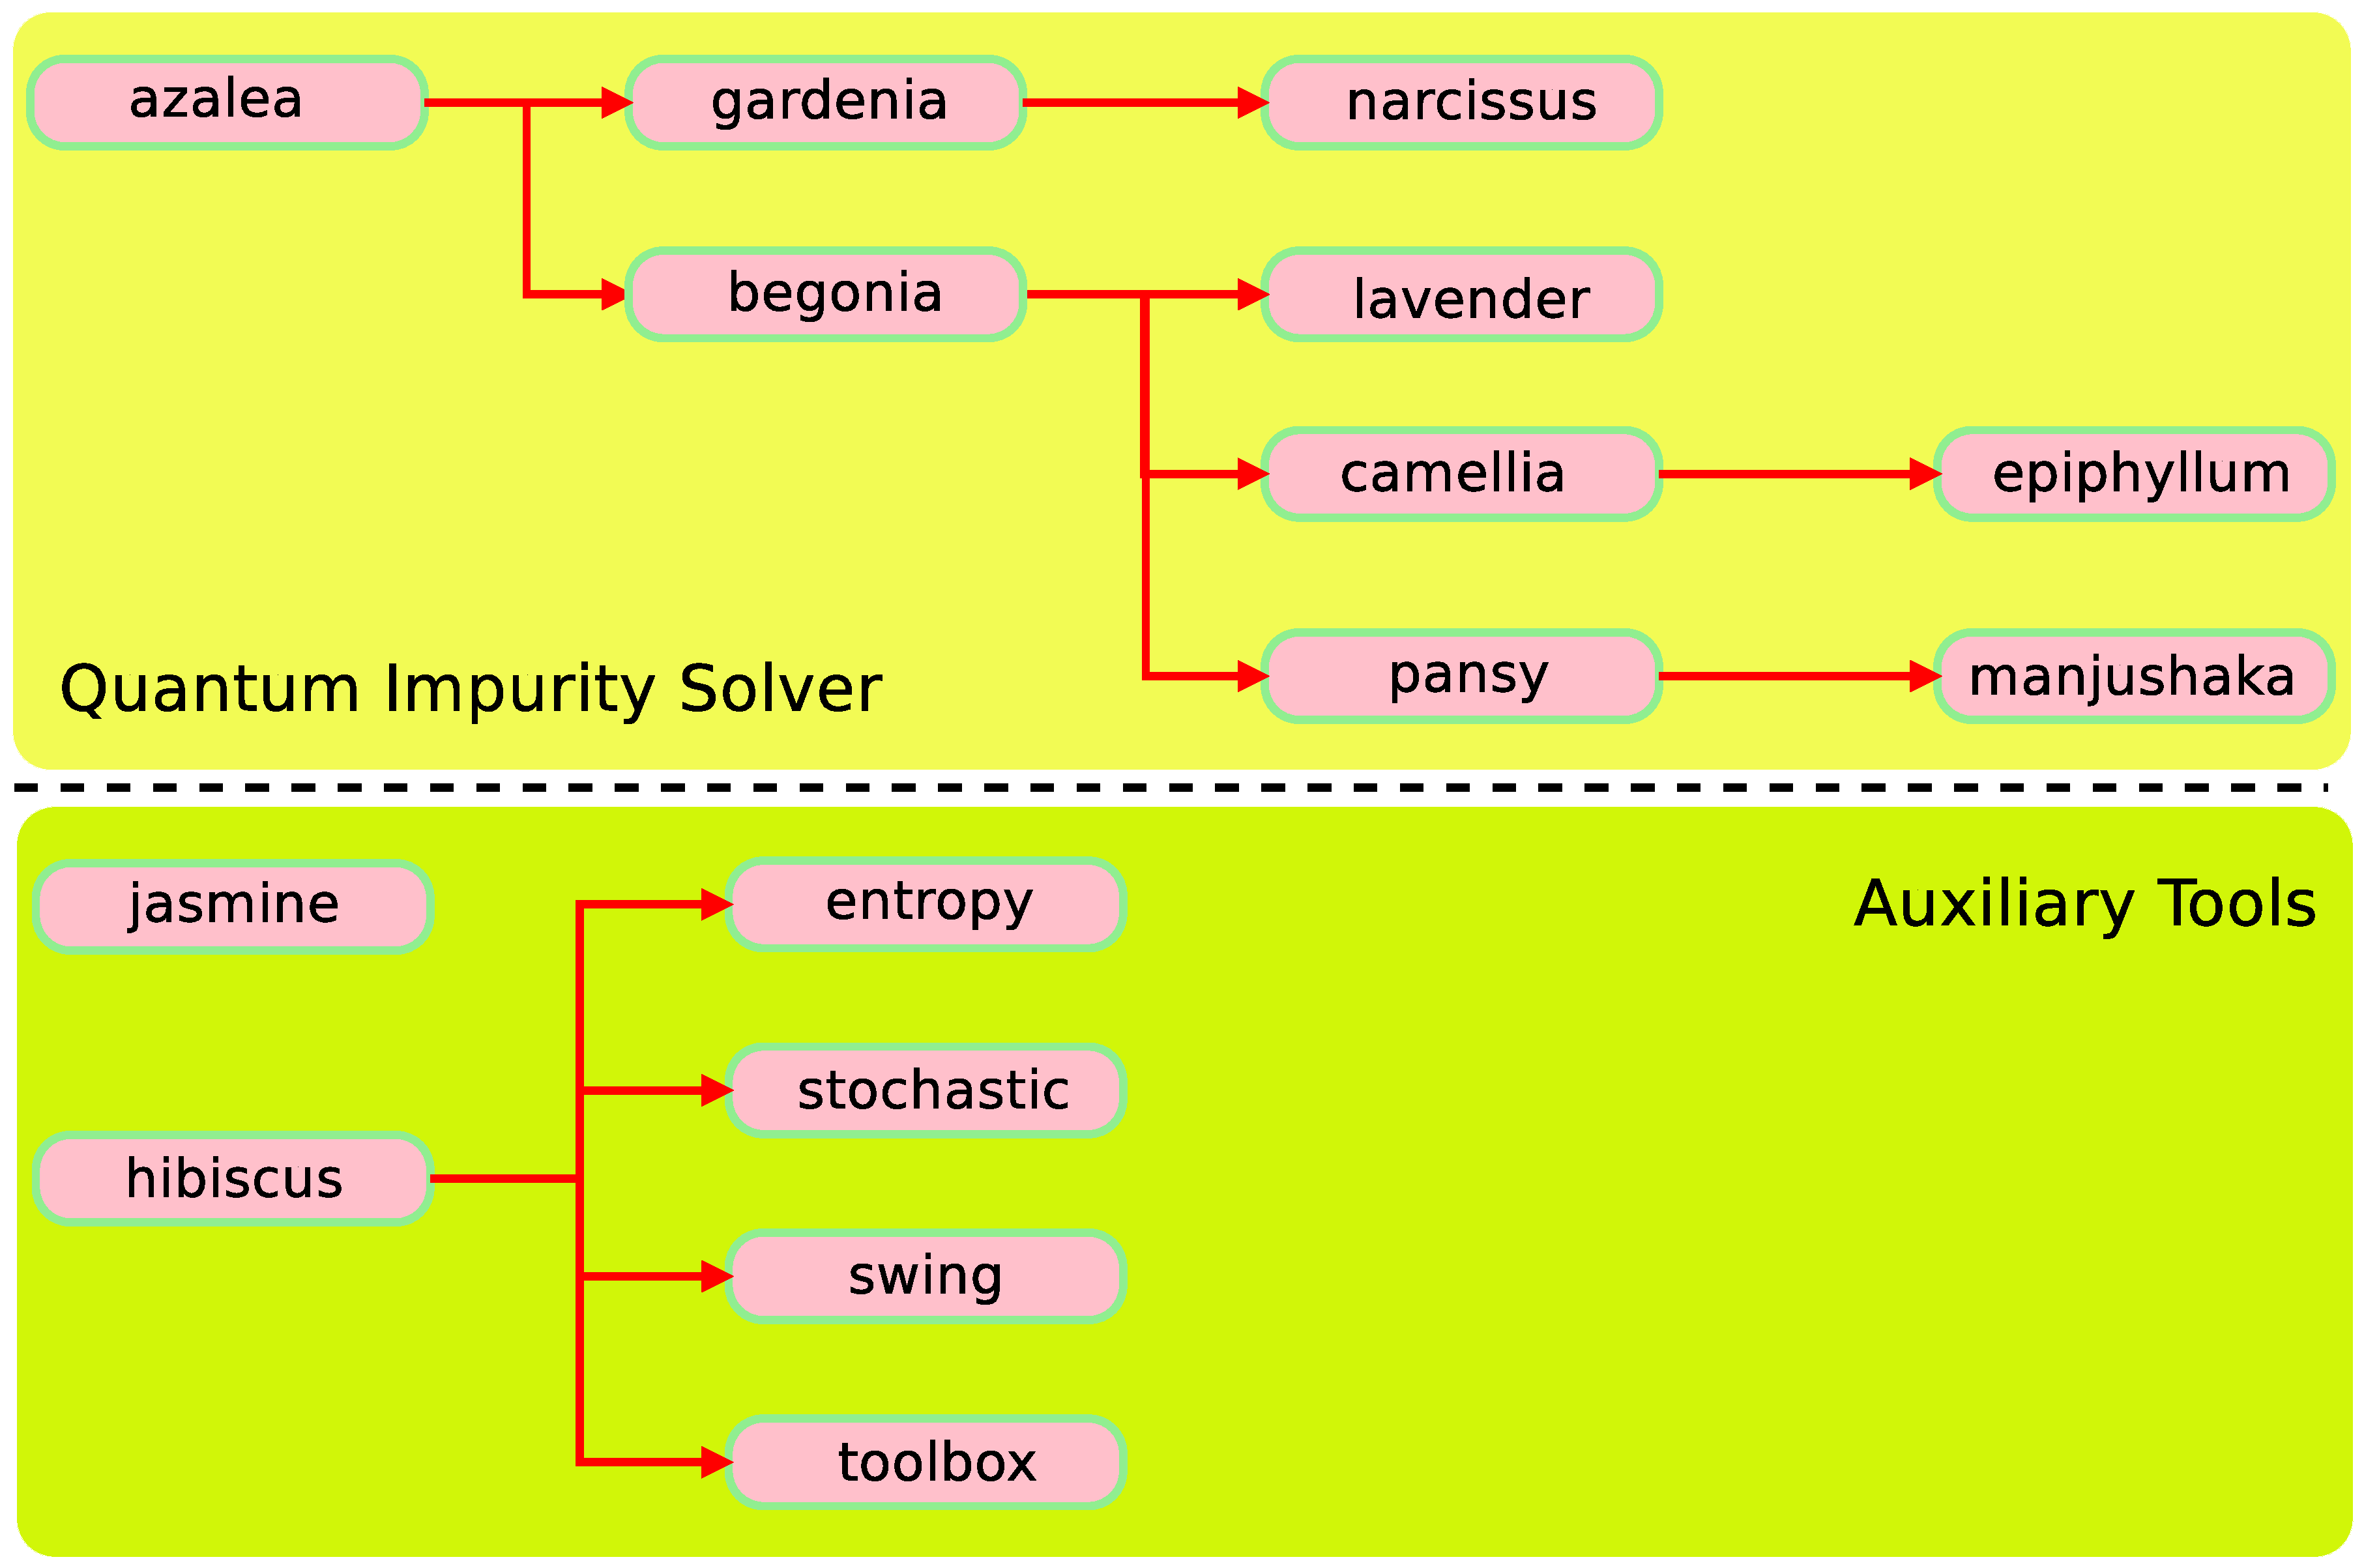
\includegraphics[scale=0.24]{figure/history.eps}
\caption{{\iqist}软件包各组件的继承关系\label{fig:history}}
\end{figure}

\subsubsection{{\azalea}}

{\azalea}是采用CT-HYB算法的连续时间量子蒙特卡洛杂质求解器,是所有CT-QMC杂质求解器的原型,也是
{\iqist}中第一个开发完毕的连续时间量子蒙特卡洛杂质求解器。该杂质求解器基于segment表象算
法\cite{werner:076405},仅仅支持具有密度$-$密度相互作用形式的哈密顿量,运行性能极其稳定高效。

\subsubsection{{\gardenia}}
{\gardenia}是采用CT-HYB算法的连续时间量子蒙特卡洛杂质求解器,它是在{\azalea}的基础之上发展而
来。它相对于{\azalea}的最大改进就是可以选择采用正交多项式表象以及内核多项式表象\cite{ortho:075145}来改善电子自能
函数以及虚时格林函数的测量精度。同时{\gardenia}的功能也大为扩充了,能够测量自旋$-$自旋关联函
数、轨道$-$轨道关联函数、双粒子格林函数以及顶角函数等等。{\gardenia}的运行效率要明显弱于{\azalea},但
是相对于Hirsch-Fye算法(亦即{\daisy}组件)而言,仍属十分高效。

\subsubsection{{\narcissus}}
{\narcissus}是采用CT-HYB算法的连续时间量子蒙特卡洛杂质求解器,它是在{\gardenia}的基础之上发展
而来。它相对于{\gardenia}的最大改进是支持动态屏蔽效应\cite{werner:2010}以及Hubbard-Holstein模
型\cite{werner:146404}的计算。但是在{\narcissus}中不再支持{\gardenia}与{\azalea}杂质求解器都支
持的GLOBAL SWAP算法\footnote{该算法由戴希研究员提出。},这意味着{\narcissus}杂质求解器不支持研
究极端高温体系。在考虑动态屏蔽效应或是研究Hubbard-Holstein模型时,{\narcissus}的运行效率要明显弱于
{\gardenia}。但是在研究普通系统时,{\narcissus}、{\gardenia}与{\azalea}组件的运行效率没有明显
的差别。总体而言,在运行效率方面,{\azalea} $\geq$ {\gardenia} $\geq$ {\narcissus}。

\subsubsection{{\begonia}}
{\begonia}是采用CT-HYB算法的连续时间量子蒙特卡洛杂质求解器,它也是在{\azalea}的基础之上发展而
来。该杂质求解器基于广义矩阵表象\cite{werner:155107},支持任意相互作用形式的哈密顿量,运行性能较之{\azalea}有较大
的降低。{\begonia}采用了稀疏矩阵技术以及分而治之的策略来提高计算效率,但是并没有采用好量子数
以及分块矩阵乘法技术\cite{haule:155113},因此{\begonia}并不适用于研究较大的体系,五带模型就是它的极限了。

\subsubsection{{\lavender}}
{\lavender}是采用CT-HYB算法的连续时间量子蒙特卡洛杂质求解器,它是在{\begonia}的基础之上发展而
来。它相对于{\begonia}的最大改进就是可以选择采用正交多项式表象以及内核多项式表象\cite{ortho:075145}来改善虚时格林
函数的测量精度。同时{\lavender}还支持双粒子格林函数以及顶角函数的测量。经过修正的{\lavender}还
可以用于研究含自旋$-$轨道耦合效应的系统。同{\begonia}类似,{\lavender}也不适用于研究较大的体系,
五带Hubbard模型是它的极限。

\subsubsection{{\jasmine}}
{\jasmine}是前处理程序,主要作用是对角化原子问题,产生atom.cix文件,与{\begonia}、{\lavender}、{\camellia}、
{\epiphyllum}、{\pansy}、{\manjushaka}等程序配合使用。目前{\jasmine}并不支持自旋$-$轨道耦合效应(SOC),
如果用户的模型需要考虑SOC,那么必须采用杜亮博士提供的专用版本的rambutan程序。

\subsubsection{{\hibiscus}}
{\hibiscus}是一大类前处理与后处理程序的集合,须与各种量子蒙特卡洛杂质求解器配合使用。它包含
entropy、stochastic、swing与toolbox等四个组件。其中entropy组件是最大熵程序\cite{jarrell:133},用于虚时
格林函数的解析延拓\footnote{即由$G(\tau)$得到$G(\omega)$。}。stochastic组件是随机解析延拓程序\cite{beach},
同样用于虚时格林函数的解析延拓。swing组件用于电子自能函数的解析延拓\footnote{即由$\Sigma(i\omega)$得
到$\Sigma(\omega)$。}。toolbox组件包含了十余个前/后处理小程序。

\section{{\iqist}的主要功能}
\label{sec:function}

{\iqist}项目的主要开发语言为Fortran 90语言,有部分后处理程序应用了Python\footnote{指{\hibiscus}组件中的
swing程序。}。开发平台为GNU/Linux系统,采用Bazzar版本控制软件来控制开发进程。{\iqist}的主要程序均支持MPI
并行计算,所有程序都经过了高度的优化,追求运行速度的极限。{\iqist}的主要程序均经过反复测试,其可靠性也得
到多次验证。

{\iqist}的量子杂质求解器组件\footnote{仅指基于CT-HYB算法的量子杂质求解器组件,因此{\daisy}与{\sakura}组
件不包括在内。}可以求解如下的量子杂质模型:
\begin{itemize}
\item 1 $\sim$ 7 带Hubbard模型 ({\begonia}与{\lavender}仅仅支持五带及五带以下的系统)
\item 任意强度的Coulomb相互作用$U$以及Hund交换作用$J$
\item 动态屏蔽效应 (仅仅{\narcissus}支持)
\item Hubbard-Holstein模型 (仅仅{\narcissus}支持)
\item Bethe晶格,可扩充至其它晶格模型
\item 密度$-$密度相互作用
\item 具有旋转不变性的广义相互作用 (除了{\azalea}、{\gardenia}与{\narcissus}外均支持)
\item 自旋$-$轨道耦合作用 (仅仅{\lavender}支持\footnote{源程序需要进行额外的修改。})
\item 系统温度 $0.5 < \beta < 400$ (仅仅{\azalea}与{\gardenia}支持$\beta < 5$)
\item Krylov子空间迭代算法(仅仅{\camellia}与{\epiphyllum}支持)
\item Newton-Leja多项式插值算法(仅仅{\camellia}与{\epiphyllum}支持)
\item 子空间分块算法(仅仅{\pansy}与{\manjushaka}支持)
\item 正交多项式算法(除了{\azalea}、{\begonia}与{\pansy}外均支持)
\item 内核多项式算法(除了{\azalea}、{\begonia}与{\pansy}外均支持)
\item MPI并行加速
\item OpenMP并行加速(仅仅{\epiphyllum}支持)
\item 可独立运行也可与LDA + DMFT接口程序联用
\end{itemize}

{\iqist}的量子杂质求解器组件\footnote{仅指基于CT-HYB算法的量子杂质求解器组件,因此{\daisy}与{\sakura}组
件不包括在内。}可以输出如下的观测量:
\begin{itemize}
\item 虚时格林函数$G(\tau)$,虚频格林函数$G(i\omega)$
\item 虚时weiss函数$\mathcal{G}(\tau)$,虚频weiss函数$\mathcal{G}(i\omega)$
\item 虚时杂化函数$\Delta(\tau)$,虚频杂化函数$\Delta(i\omega)$
\item 虚频自能函数$\Sigma(i\omega)$
\item 原子虚频格林函数$G_{\text{atom}}(i\omega)$,原子虚频自能函数$\Sigma_{\text{atom}}(i\omega)$
\item 轨道占据数$\langle n_{\alpha} \rangle$,双占据数$\langle n_{\alpha} n_{\beta} \rangle$
\item 动能$E_{\text{kin}}$、势能$E_{\text{pot}}$、总能$E_{\text{tot}}$、平均有效磁矩$\langle S_{z} \rangle$
\item 微扰展开项分布概率$P_{\text{H}}$
\item 原子组态分布概率 $P_{\Gamma}$
\item 自旋$-$自旋关联函数$\langle S_{z}(0) S_{z}(\tau) \rangle$ (仅仅{\gardenia}与{\narcissus}支持)
\item 轨道$-$轨道关联函数$\langle N_{\alpha}(0) N_{\alpha}(\tau) \rangle$ (仅仅{\gardenia}与{\narcissus}支持)
\item 双粒子虚时格林函数$g_{2}$ (仅仅{\gardenia}, {\narcissus}与{\lavender}支持)
\item 顶角函数$\gamma_{4}$ (仅仅{\gardenia}, {\narcissus}与{\lavender}支持)
\end{itemize}

\section{{\iqist}的版本历史}
\label{sec:history}

v0.01, 2004年, 开始项目初始开发。

v0.02, 2005年,实现单带Hirsch-Fye量子蒙特卡洛杂质求解器。

v0.03, 2006年,实现多带Hirsch-Fye量子蒙特卡洛杂质求解器, {\daisy}组件的前身。

v0.04, 2007年, 实现弱耦合连续时间量子蒙特卡洛杂质求解器,{\sakura}组件的前身。

v0.05, 2009年,实现强耦合连续时间量子蒙特卡洛杂质求解器,{\azalea}组件与{\hibiscus}组件。

v0.06, 2010年,实现强耦合连续时间量子蒙特卡洛杂质求解器, {\begonia}组件与{\jasmine}组件。

v0.07, 2011年,实现了{\gardenia}、{\narcissus}与{\lavender}等组件。

v0.10, 2012年8月,提出创建{\iqist} 软件包,开始编写本文档。

v0.11, 2012年10月,用户文档基本成型。

v0.12, 2012年11月,用户文档分发相关用户修订校阅。

v0.13,2012年12月,{\iqist}软件包基本成型,准备公开发布。

\section{{\iqist}的使用条款}
\label{sec:license}

如果你需要使用{\iqist},那么必须遵守如下用户条款(十分宽松的,不必担心):

\begin{itemize}
\item {\iqist}是开源软件,用户可以自由编译、链接、使用、复制、拷贝、分发、修改、破坏、删除它。
\item 用户可以任意修改、复制、调用{\iqist}的代码片段或者是函数。
\item 如果用户修改了{\iqist}的源代码,希望能及时反馈回开发者处。
\item 如果用户发现了任何的bug,或者是有任何的建议,欢迎与开发者联系。
\item 如果用户需要在{\iqist}的基础上重新发布修改过的程序,那么禁止使用{\iqist}或者是类似的名称。
\item 尽管开发者对{\iqist}的可靠性有足够的信心,但是开发者并不能保证计算结果的绝对正确性。
\item 开发者一般不对用户提供无偿的技术支持。
\item 对于用户使用{\iqist}所造成的任何直接/间接后果,开发者一概不予负责。
\item 如果用户在工作中使用了{\iqist},希望能够引用如下的论文或者是把开发者列为共同作者。

\noindent\colorbox{pink}{\parbox[r]{\linewidth}{Li Huang, Yilin Wang, Liang Du and Xi Dai, \\ 
User's Guide for Interacting Quantum Impurity Systems Simulating Toolkit, 2012 }}

\item 上述条款的最终解释权为黄理(huangli712@gmail.com)所有。
\end{itemize}
